\newpage
\chapter{Resultaten}

\section{Soorten netwerken}

\textit{In dit hoofdstuk wordt er onderzocht welke verschillende netwerken er gebruikt worden in bestaande implementaties. Hierbij wordt zowel de definitie van soorten en de selectie van implementaties gebruikt uit de resultaten van het vooronderzoek.}

"De distributie van informatie en het probleem van wederzijdse overeenstemming over een consistente staat van het netwerk vormt een uitdaging, zeker in de aanwezigheid van zelfzuchtige en/of kwaadwillende deelnemers" - \citet{7423672}. Het is een uitdaging die bekend staat als het Byzantine Generals' Problem, en is beschreven door \citet{lamport1982byzantine}. Het stelt dat het essentieel is voor een betrouwbaar computersysteem om te kunnen gaan met fouten die optreden in een of meer van de componenten, waardoor het kan voorkomen dat er conflicterende informatie verstuurd wordt naar de andere componenten van het systeem. In hoeverre een computersysteem hiermee om kan gaan wordt de \acrfull{BFT} genoemd en wordt aangeduid als: $ f = [\frac{N - 1}{t}] $ waarbij \(N\) componenten van een computersysteem zijn en \(t\) de foutieve componenten.

In blockchain implementaties zijn de componenten die onbetrouwbaar zijn de deelnemers van het peer-to-peer netwerk. Het soort netwerk is dan ook verbonden met de manier waarop consensus bereikt wordt tussen de deelnemers van het netwerk en is getypeerd als het consensus protocol dat geïmplementeerd is.

\newpage

\subsection{Proof of Work}
\label{chapter-proof-of-work}
De originele implementatie van Blockchain technologie is gepresenteerd door \citet{nakamoto2008bitcoin} in \textit{"Bitcoin: A peer-to-peer electronic cash system"}. Het maakt gebruik van een algoritme genaamd \acrfull{PoW} om consensus te bereiken. Hierbij gaat het om het oplossen van een wiskundig probleem $Y \in \mathbb{N} < f(X + n)$ waarbij $f$ een hash functie is, $n$ de \gls{nonce}, $X$ de data en $Y$ de \gls{difficulty}.

\begin{wrapfigure}{r}{0.5\textwidth}
  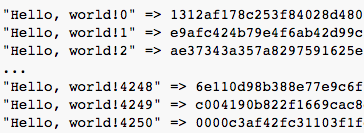
\includegraphics[width=0.5\textwidth, height=25mm]{proof-of-work}
  \caption[Proof-of-Work in Bitcoin]{Werking Proof-of-Work, van \citet{ProofofWork}. Wanneer de eerste vier bits ($Y = 4$) van de hash 0 zijn is de proef opgelost. }
  \label{proof-of-work}    
\end{wrapfigure}
In het geval van Bitcoin is de $Y$ waarde een getal die aanduid wat de \gls{difficulty} is om de hash te berekenen en wordt de $X$ waarde incrementeel opgehoogd. Een voorbeeld is gegeven in fig. \ref{proof-of-work}. Dit proces zorgt ervoor dat de integriteit van de data in een block op de Blockchain bewaakt wordt. Wanneer een kwaadwillende deelnemer aan het netwerk de data van een block wilt aanpassen die reeds opgenomen is in de Blockchain, kan er via het \acrshort{PoW} makkelijk gevalideerd worden of het block invalide is.

Daarnaast beschrijft de bedenker van het protocol, Satoshi Nakamoto, het \acrshort{PoW} algoritme als 'one-CPU-one-vote'. Aangezien het gebruikte hashing algoritme geen limitaties stelt tot de zogeheten \gls{voting_power} van een deelnemer in het netwerk creëert het gunstige omstandigheden voor high-end GPU eigenaren tegenover high-end CPU eigenaren \citep[p.~2]{van2013cryptonote}.

\textbf{Monero} maakt gebruik van het CryptoNight algoritme \citep{noether2014monero}, een implementatie gebaseerd op CryptoNote, waarin gebruik gemaakt wordt van een egalitair Proof of Work \citep[p.~11]{van2013cryptonote}. In contrast met het Bitcoin protocol Proof of Work algoritme is het ontworpen om inefficiënt berekenbaar te zijn op een GPU, waardoor er gelijke kansen zijn voor de deelnemers van het netwerk die het mining proces uitvoeren.

\newpage
\subsection{Proof of Stake}

"Een eerste overweging met betrekking tot de werking van blockchain protocollen gebaseerd op Proof of Work -- zoals Bitcoin -- is de energie benodigd voor hun uitvoering." - \citet{kiayias2017ouroboros}.
In een onderzoek gedaan door \citeauthor{ODwyer:Bitcoin} in \citeyear{ODwyer:Bitcoin} naar het energieverbruik van het Bitcoin mining netwerk is geschat dat onder redelijke omstandigheden het netwerk gelijk stond met het energiegebruik van Ierland. Om deze reden zijn er onderzoeken en experimenten gedaan naar alternatieve consensus algoritmes. \acrfull{PoS} is een consensus algoritme waarbij, in plaats van het verspillen van elektriciteit om zware rekenkundige problemen op te lossen, een deelnemer geselecteerd wordt om het volgende blok te genereren (doorgaans \gls{minting} genoemd) op basis van willekeurige selectie en rijkdom of leeftijd (i.e., de stake).

\paragraph{Cardano} maakt gebruik van \acrshort{PoS} waarbij iedere deelnemer van het netwerk met een positief balans (e.g. stake) als stakeholders gezien worden. Om uitgekozen te worden om een nieuw block te genereren moet een stakeholder geselecteerd worden als \gls{slot_leader}. De implementatie verdeelt de fysieke tijd in tijdvakken en elke tijdvak is verdeeld in slots. Voor elke slot wordt een \gls{slot_leader} verkozen, die verantwoordelijk is voor het produceren van één blok. Niet alle deelnemers van het netwerk, bijvoorbeeld die minder dan 2\% van de totale circulatie van \glspl{token} hebben, worden geselecteerd om benoemd te worden tot \gls{slot_leader}. Deze groep van deelnemers maken deel uit van de \glspl{elector} groep. \Glspl{elector} verkiezen nieuwe \glspl{slot_leader} gedurende het huidige tijdsvak, waarna er een selectie gemaakt wordt en de nieuwe \glspl{slot_leader} vaststaan voor het volgende tijdsvak. Hoe meer \gls{stake} een deelnemer heeft, hoe groter de kans dat zij uitgekozen wordt om een \gls{slot_leader} te worden in het volgende tijdsvak. De \gls{slot_leader} luistert naar transacties die aangekondigd worden door andere nodes, bundelt ze in een nieuw block, signeert het met zijn private key en publiceert het block in het netwerk \citep{cardano_wiki:proof_of_stake}.

\paragraph{EOS} is een implementatie die gebruik maakt van \acrfull{DPoS} om consensus te bereiken. Het grote verschil tussen \acrshort{DPoS} en \acrshort{PoS}; in een \acrshort{PoS} systeem is elke deelnemer die \gls{stake} heeft maakt onderdeel uitmaken van het validatie- en consensusproces. Met \acrshort{DPoS} kan elke deelnemer die \gls{stake} heeft andere deelnemers verkiezen die onderdeel uitmaken van het validatie- en consensusproces \citep{steemit:eos_dpos}. In contrast met het \acrshort{PoW} algoritme is er geen competitie voor het produceren van een block, maar wordt er samengewerkt om een block te produceren.

\newpage
\section{Gevaren}

Wanneer deelnemers uitmaken van een grootschalig netwerk die niet gecontroleerd wordt door een centrale autoriteit kan het voorkomen dat deelnemers zich misdragen. In juli 2016 is Ethereum opgesplitst in twee partities die dezelfde valuta hanteren; \textit{Ethereum} en \textit{Ethereum Classic}. Dit is veroorzaakt door een kwaadwillende deelnemer in het netwerk die door een bug in het systeem geld naar zichzelf toe kon sturen. Dit heeft ertoe geleid dat veel gebruikers mogelijk een aanzienlijk verlies geleden hebben, waaronder veel ontwikkelaars van Ethereum. Om dit verlies op te lossen werd er een hard-fork voorgesteld die Ethereums code aanpast waarbij de transacties van de kwaadwillende deelnemer teruggedraaid werden \citep{kiffer2017stick}. 

Dit illustreert een van de mogelijke manieren waarop een kwaadwillende gebruiker het systeem kan ondermijnen. Om een duidelijk overzicht te geven van de gevaren binnen een gedecentralizeerd peer-to-peer systeem wordt er onderzocht welke technieken toegepast worden om aanvallen van een kwaadwillende deelnemer van het netwerk tegen te gaan.

\subsection{Eclipse Attack}
Een aanval op het peer-to-peer netwerk waarbij er controle over een deelnemer zijn toegang tot informatie gelimiteerd, of zelfs gemanipuleerd wordt. Met de juiste manipulatie van het peer-to-peer netwerk kan er informatie verduistert worden zodat een goedwillende deelnemer aan het netwerk alleen maar kan communiceren met kwaadwillende deelnemers. Dit kan leiden tot \gls{block_races}, \gls{selfish_mining} en \gls{0-confirmation_double_spending} \citep{heilman2015eclipse}.

\subsection{Majority Attack}
Een aanval waarbij één deelnemer de richting van het netwerk bepaald door het bezitten van 51\% de \gls{voting_power}. In het geval van \acrlong{PoW} betekend dit dat de kwaadwillende deelnemer 51\% van de totale rekenkracht nodig heeft om deze aanval uit te voeren. Dit stelt de kwaadwillende deelnemer in staat om het netwerk te manipuleren en kan leiden tot \gls{0-confirmation_double_spending}.

\subsection{\acrfull{DoS}}
Een algemene benaming voor een collectie van mogelijke oorzaken voor een bewuste verstoring van de services die het peer-to-peer netwerk faciliteert. Dit kan op meerdere manieren optreden, bijvoorbeeld door het invoegen van heel veel transacties in één block, zodat het lang duurt voordat het peer-to-peer netwerk het nieuwe block heeft opgenomen.

\subsection{Sybil Attack}
Een aanval waarbij een deelnemer meerdere virtuele deelnemers creëert in het netwerk waarbij de gecreëerde deelnemers het verkiezingsproces kunnen verstoren door verkeerde informatie door te geven in het netwerk, zoals positief stemmen voor een malafide transactie \citep{conti2017survey}.

\subsection{Double spending}
Bij Creditcard-gebaseerde betalingen wordt er eerlijkheid bereikt door het bestaan van een bank of een andere vertrouwde tussenpersoon (e.g. Paypal). Hierbij wordt de tussenpersoon vertrouwd om te controleren dat diegene die een betaling doet aan een derde partij het geld niet al heeft uitgegeven \citep{karame2012two}. In gedecentralizeerde systemen, waarbij er geen vertrouwe tussenpersoon aanwezig is, staat dit bekend als het \textit{double spending} probleem, waarbij het mogelijk is om \glspl{token} die reeds uitgegeven zijn (i.e. opgenomen in een block) nogmaals gebruikt wordt om een transactie uit te voeren. 

\subsection{Nothing at Stake}
Wanneer er een \gls{fork} ontstaat is de optimale strategie elke replica van de blockchain te valideren, zodat de diegene die het validatie proces uitvoert nog steeds uitbetaald krijgt, ongeacht of de \gls{fork} geaccepteerd wordt of niet.

\newpage

\section{Identiteit}

Blockchain kan een zeker mate van privacy garanderen door de public en private keys, wat ervoor zorgt dat een gebruiker niet zijn echte identiteit hoeft te hanteren om met het systeem te interacteren. Echter, \cite{meiklejohn2013fistful} toont aan dat blockchain niet de transactionele privacy kan waarborgen omdat de waarden van alle transacties en saldo van elke public key openbaar inzichtbaar zijn.

\citet{Okamoto:1991:UEC:646756.705374} beschrijft zes criteria waaraan de ideale implementatie van elektronisch geld moet voldoen. In het bijzonder worden er twee criteria genoemd:

\begin{itemize}
  \item \textbf{Untraceability:} voor elke inkomende transactie hebben alle mogelijke afzenders gelijke kansen om geïdentificeerd te worden als verstuurder. 
  
  \item \textbf{Unlinkability:} voor elke twee uitgaande transacties moet het onmogelijk zijn om aan te tonen dat ze naar dezelfde persoon verstuurd zijn.
\end{itemize}

\newpage

\section{Bitcoin}
\subsection{Functionaliteit}
\paragraph{Architectuur}
Bitcoin is een netwerk waarin geen coördinerende rollen zijn. Elke deelnemer van het netwerk heeft een complete replica van alle informatie die benodigd is voor het verifiëren van de validiteit van binnenkomende transacties. Er zijn verschillende services die het netwerk faciliteert die kort toegelicht zijn in \ref{blockchain_node_types}, twee daarvan zijn met name belangrijk voor de beschrijving van het netwerk: netwerk routing, en het mining proces. In de basis van het netwerk staan de transacties die op abstract niveau bitcoins van een of meer accounts naar een of meer bestemmingsaccounts overmaken. Een \gls{account}, in de context van het bitcoin netwerk, is een combinatie van een public- en private key, waarbij de public key als identificatie van de \gls{account} gebruikt wordt. Om een transactie te versturen wordt de transactie gesigneerd met de private key van de \gls{account} die de transactie wilt uitvoeren. 
\begin{wrapfigure}{r}{0.6\textwidth}
  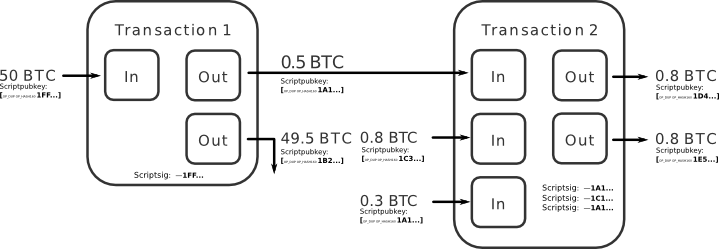
\includegraphics[width=0.6\textwidth]{utxo}
  \caption[UTXO-model]{Voorbeeld van het UTXO-model zoals in gebruik bij Bitcoin, bron: http://news.8btc.com/thoughts-on-bytom-design-extension-of-utxo-structure.}
  \label{utxo_model}
\end{wrapfigure}

Transacties bestaan uit een input en output. In plaats van het aggregeren van een balans voor elk \gls{account}, wordt er bijgehouden wat de output van een transactie is. De balans is hierbij de som van alle openstaande outputs van het desbetreffend \gls{account}. In fig. \ref{utxo_model} is te zien hoe dit in zijn werk gaat. Een onderdeel van de services die de \glspl{node} binnen het netwerk aanbieden is het valideren van transacties. Hierbij worden drie onderdelen gevalideerd:

\begin{itemize}

  \item Een output mag maar één keer geclaimd zijn.
  \item Nieuwe outputs worden alleen gecreëerd door een transactie.
  \item De som van alle waardes van de geclaimde outputs moet groter zijn als de totale som van de nieuwe gecreëerde outputs.
\end{itemize}

Wanneer dit het geval is wordt de transactie geaccepteerd en opgenomen in de lokale replica van de blockchain. Over tijd kan het voorkomen dat de replica van verschillende \glspl{node} inconsistent worden, waarbij het kan voorkomen dat er twee of meer transacties dezelfde coin meerdere malen uitgeeft. Dit staat bekend als \gls{double_spending} \citep{6688704}.

\clearpage
Een nieuw block wordt gecreëerd door het uitvoeren van het mining proces. Dit wordt uitgevoerd door zogenaamde \glspl{miner} node. Om te bepalen welke \gls{node} verantwoordelijk is voor het volgende block moet er een oplossing gevonden worden voor het proof-of-work. Dit proces zorgt ervoor dat er een beslissing gemaakt wordt over de volgorde van de transacties, en dat de inhoudt van een block niet aangepast kan worden omdat dit in directe verbinding staat met het gedane \acrshort{PoW}.

\paragraph{Discovery protocol}

Om het het netwerk te betreden worden er DNS servers benaderd waarbij gebruik wordt gemaakt van het TCP protocol. Deze DNS servers worden in stand gehouden door vrijwilligers en geven een willekeurige set aan \glspl{bootstrap_node} terug die actief zijn in het netwerk. Wanneer de \gls{node} toegetreden is tot het netwerk wordt er een \gls{peer_list} bijgehouden met alle \glspl{node} waarmee er connectie is gelegd. Deze \gls{peer_list} wordt gebruikt om connectie te leggen bij een eerstvolgende toetreding tot het netwerk.

\paragraph{Informatie propagatie}

Voor het updaten en synchroniseren van de blockchain worden er \acrfull{tx} en block berichten verstuurd. Om tegen te gaan dat \acrshort{tx}- en block berichten verstuurd worden naar \glspl{node} die al afweten van deze informatie, wordt er een \textit{inv} bericht verstuurd wanneer een transactie of een block volledig geverifieerd is. Het \textit{inv} bericht bevat een lijst van transactie- en block hashes die reeds ontvangen zijn door de verstuurder en die beschikbaar zijn om opgehaald te worden. 
\begin{wrapfigure}{r}{0.5\textwidth}
  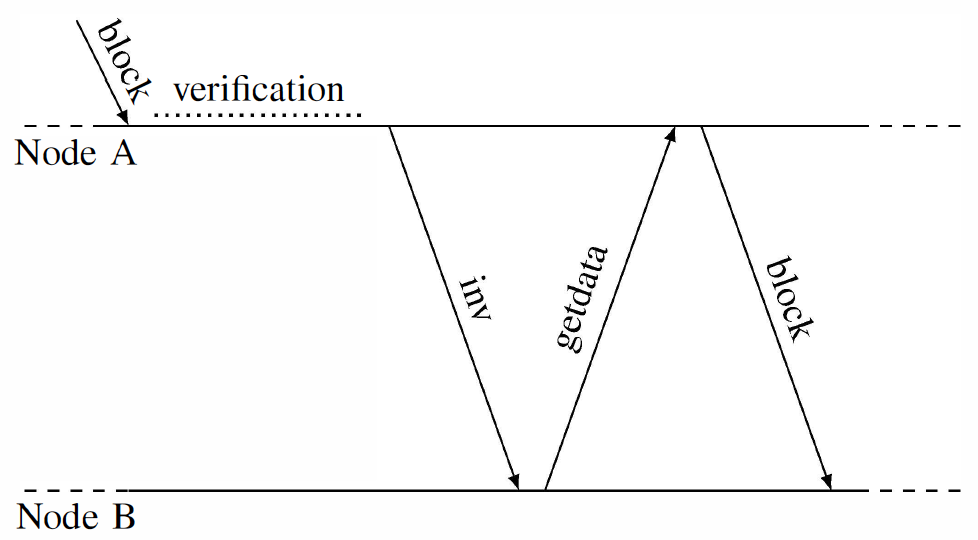
\includegraphics[width=0.5\textwidth]{bitcoin_information_propagation_0}
  \caption[Communicatie tussen deelnemers in Bitcoin]{Berichten die verzonden worden om informatie over een block uit te wisselen \citep[p.~4]{6688704}.}
  \label{bitcoin_information_propagation_0}
\end{wrapfigure}

Wanneer een \gls{node} deze informatie wilt ontvangen (bijv. omdat het de informatie nog niet heeft), wordt er een \textit{getdata} bericht verstuurd naar de verstuurder van het \textit{inv} bericht, met daarin de hashes van de informatie die de \gls{node} wilt hebben. Fig. \ref{bitcoin_information_propagation_0} visualiseert dit proces.
\subsection{Gevaren}
\paragraph{Architectuur}
Bitcoin is een netwerk waarin geen coördinerende rollen zijn. Elke deelnemer van het netwerk heeft een complete replica van alle informatie die benodigd is voor het verifiëren van de validiteit van binnenkomende transacties. Er zijn verschillende services die het netwerk faciliteert die kort toegelicht zijn in \ref{blockchain_node_types}, twee daarvan zijn met name belangrijk voor de beschrijving van het netwerk: netwerk routing, en het mining proces. In de basis van het netwerk staan de transacties die op abstract niveau bitcoins van een of meer accounts naar een of meer bestemmingsaccounts overmaken. Een \gls{account}, in de context van het bitcoin netwerk, is een combinatie van een public- en private key, waarbij de public key als identificatie van de \gls{account} gebruikt wordt. Om een transactie te versturen wordt de transactie gesigneerd met de private key van de \gls{account} die de transactie wilt uitvoeren. 
\begin{wrapfigure}{r}{0.6\textwidth}
  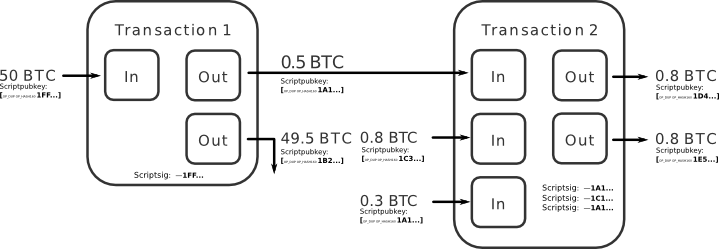
\includegraphics[width=0.6\textwidth]{utxo}
  \caption[UTXO-model]{Voorbeeld van het UTXO-model zoals in gebruik bij Bitcoin, bron: http://news.8btc.com/thoughts-on-bytom-design-extension-of-utxo-structure.}
  \label{utxo_model}
\end{wrapfigure}

Transacties bestaan uit een input en output. In plaats van het aggregeren van een balans voor elk \gls{account}, wordt er bijgehouden wat de output van een transactie is. De balans is hierbij de som van alle openstaande outputs van het desbetreffend \gls{account}. In fig. \ref{utxo_model} is te zien hoe dit in zijn werk gaat. Een onderdeel van de services die de \glspl{node} binnen het netwerk aanbieden is het valideren van transacties. Hierbij worden drie onderdelen gevalideerd:

\begin{itemize}

  \item Een output mag maar één keer geclaimd zijn.
  \item Nieuwe outputs worden alleen gecreëerd door een transactie.
  \item De som van alle waardes van de geclaimde outputs moet groter zijn als de totale som van de nieuwe gecreëerde outputs.
\end{itemize}

Wanneer dit het geval is wordt de transactie geaccepteerd en opgenomen in de lokale replica van de blockchain. Over tijd kan het voorkomen dat de replica van verschillende \glspl{node} inconsistent worden, waarbij het kan voorkomen dat er twee of meer transacties dezelfde coin meerdere malen uitgeeft. Dit staat bekend als \gls{double_spending} \citep{6688704}.

\clearpage
Een nieuw block wordt gecreëerd door het uitvoeren van het mining proces. Dit wordt uitgevoerd door zogenaamde \glspl{miner} node. Om te bepalen welke \gls{node} verantwoordelijk is voor het volgende block moet er een oplossing gevonden worden voor het proof-of-work. Dit proces zorgt ervoor dat er een beslissing gemaakt wordt over de volgorde van de transacties, en dat de inhoudt van een block niet aangepast kan worden omdat dit in directe verbinding staat met het gedane \acrshort{PoW}.

\paragraph{Discovery protocol}

Om het het netwerk te betreden worden er DNS servers benaderd waarbij gebruik wordt gemaakt van het TCP protocol. Deze DNS servers worden in stand gehouden door vrijwilligers en geven een willekeurige set aan \glspl{bootstrap_node} terug die actief zijn in het netwerk. Wanneer de \gls{node} toegetreden is tot het netwerk wordt er een \gls{peer_list} bijgehouden met alle \glspl{node} waarmee er connectie is gelegd. Deze \gls{peer_list} wordt gebruikt om connectie te leggen bij een eerstvolgende toetreding tot het netwerk.

\paragraph{Informatie propagatie}

Voor het updaten en synchroniseren van de blockchain worden er \acrfull{tx} en block berichten verstuurd. Om tegen te gaan dat \acrshort{tx}- en block berichten verstuurd worden naar \glspl{node} die al afweten van deze informatie, wordt er een \textit{inv} bericht verstuurd wanneer een transactie of een block volledig geverifieerd is. Het \textit{inv} bericht bevat een lijst van transactie- en block hashes die reeds ontvangen zijn door de verstuurder en die beschikbaar zijn om opgehaald te worden. 
\begin{wrapfigure}{r}{0.5\textwidth}
  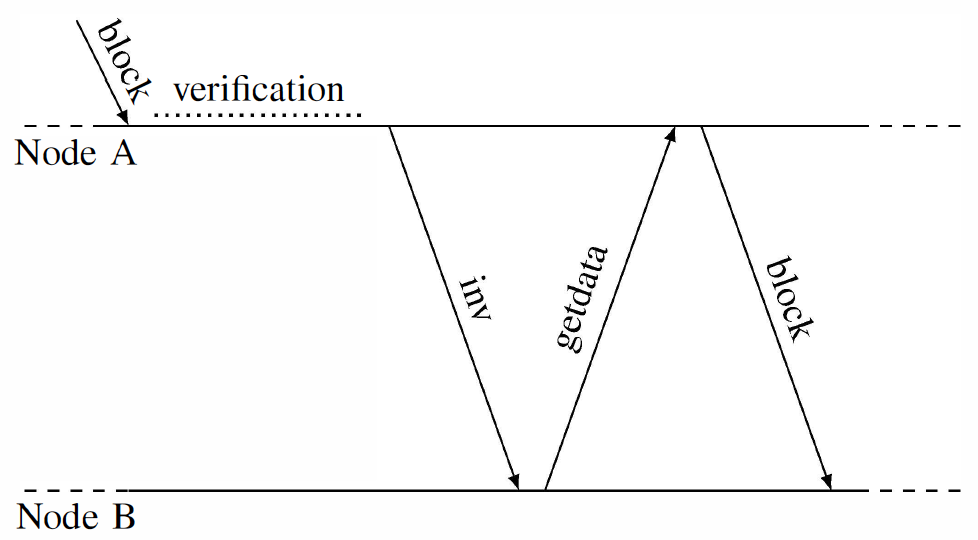
\includegraphics[width=0.5\textwidth]{bitcoin_information_propagation_0}
  \caption[Communicatie tussen deelnemers in Bitcoin]{Berichten die verzonden worden om informatie over een block uit te wisselen \citep[p.~4]{6688704}.}
  \label{bitcoin_information_propagation_0}
\end{wrapfigure}

Wanneer een \gls{node} deze informatie wilt ontvangen (bijv. omdat het de informatie nog niet heeft), wordt er een \textit{getdata} bericht verstuurd naar de verstuurder van het \textit{inv} bericht, met daarin de hashes van de informatie die de \gls{node} wilt hebben. Fig. \ref{bitcoin_information_propagation_0} visualiseert dit proces.
\subsection{Identiteit}
\paragraph{Architectuur}
Bitcoin is een netwerk waarin geen coördinerende rollen zijn. Elke deelnemer van het netwerk heeft een complete replica van alle informatie die benodigd is voor het verifiëren van de validiteit van binnenkomende transacties. Er zijn verschillende services die het netwerk faciliteert die kort toegelicht zijn in \ref{blockchain_node_types}, twee daarvan zijn met name belangrijk voor de beschrijving van het netwerk: netwerk routing, en het mining proces. In de basis van het netwerk staan de transacties die op abstract niveau bitcoins van een of meer accounts naar een of meer bestemmingsaccounts overmaken. Een \gls{account}, in de context van het bitcoin netwerk, is een combinatie van een public- en private key, waarbij de public key als identificatie van de \gls{account} gebruikt wordt. Om een transactie te versturen wordt de transactie gesigneerd met de private key van de \gls{account} die de transactie wilt uitvoeren. 
\begin{wrapfigure}{r}{0.6\textwidth}
  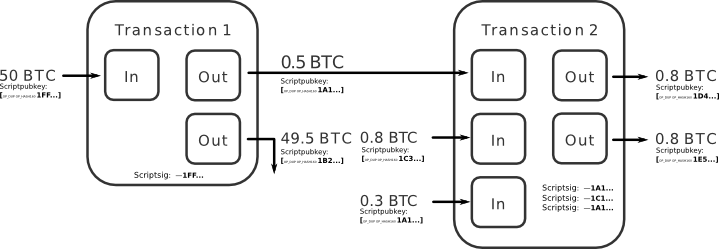
\includegraphics[width=0.6\textwidth]{utxo}
  \caption[UTXO-model]{Voorbeeld van het UTXO-model zoals in gebruik bij Bitcoin, bron: http://news.8btc.com/thoughts-on-bytom-design-extension-of-utxo-structure.}
  \label{utxo_model}
\end{wrapfigure}

Transacties bestaan uit een input en output. In plaats van het aggregeren van een balans voor elk \gls{account}, wordt er bijgehouden wat de output van een transactie is. De balans is hierbij de som van alle openstaande outputs van het desbetreffend \gls{account}. In fig. \ref{utxo_model} is te zien hoe dit in zijn werk gaat. Een onderdeel van de services die de \glspl{node} binnen het netwerk aanbieden is het valideren van transacties. Hierbij worden drie onderdelen gevalideerd:

\begin{itemize}

  \item Een output mag maar één keer geclaimd zijn.
  \item Nieuwe outputs worden alleen gecreëerd door een transactie.
  \item De som van alle waardes van de geclaimde outputs moet groter zijn als de totale som van de nieuwe gecreëerde outputs.
\end{itemize}

Wanneer dit het geval is wordt de transactie geaccepteerd en opgenomen in de lokale replica van de blockchain. Over tijd kan het voorkomen dat de replica van verschillende \glspl{node} inconsistent worden, waarbij het kan voorkomen dat er twee of meer transacties dezelfde coin meerdere malen uitgeeft. Dit staat bekend als \gls{double_spending} \citep{6688704}.

\clearpage
Een nieuw block wordt gecreëerd door het uitvoeren van het mining proces. Dit wordt uitgevoerd door zogenaamde \glspl{miner} node. Om te bepalen welke \gls{node} verantwoordelijk is voor het volgende block moet er een oplossing gevonden worden voor het proof-of-work. Dit proces zorgt ervoor dat er een beslissing gemaakt wordt over de volgorde van de transacties, en dat de inhoudt van een block niet aangepast kan worden omdat dit in directe verbinding staat met het gedane \acrshort{PoW}.

\paragraph{Discovery protocol}

Om het het netwerk te betreden worden er DNS servers benaderd waarbij gebruik wordt gemaakt van het TCP protocol. Deze DNS servers worden in stand gehouden door vrijwilligers en geven een willekeurige set aan \glspl{bootstrap_node} terug die actief zijn in het netwerk. Wanneer de \gls{node} toegetreden is tot het netwerk wordt er een \gls{peer_list} bijgehouden met alle \glspl{node} waarmee er connectie is gelegd. Deze \gls{peer_list} wordt gebruikt om connectie te leggen bij een eerstvolgende toetreding tot het netwerk.

\paragraph{Informatie propagatie}

Voor het updaten en synchroniseren van de blockchain worden er \acrfull{tx} en block berichten verstuurd. Om tegen te gaan dat \acrshort{tx}- en block berichten verstuurd worden naar \glspl{node} die al afweten van deze informatie, wordt er een \textit{inv} bericht verstuurd wanneer een transactie of een block volledig geverifieerd is. Het \textit{inv} bericht bevat een lijst van transactie- en block hashes die reeds ontvangen zijn door de verstuurder en die beschikbaar zijn om opgehaald te worden. 
\begin{wrapfigure}{r}{0.5\textwidth}
  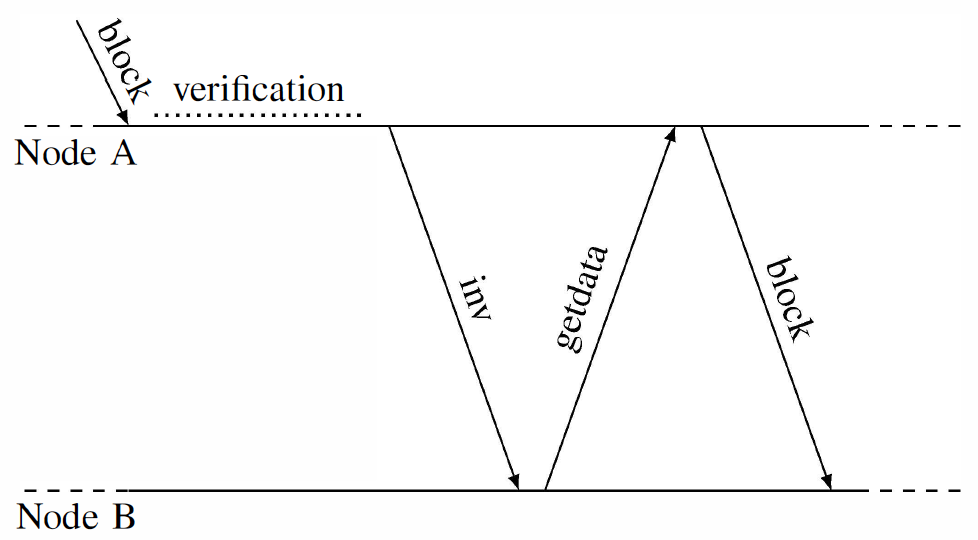
\includegraphics[width=0.5\textwidth]{bitcoin_information_propagation_0}
  \caption[Communicatie tussen deelnemers in Bitcoin]{Berichten die verzonden worden om informatie over een block uit te wisselen \citep[p.~4]{6688704}.}
  \label{bitcoin_information_propagation_0}
\end{wrapfigure}

Wanneer een \gls{node} deze informatie wilt ontvangen (bijv. omdat het de informatie nog niet heeft), wordt er een \textit{getdata} bericht verstuurd naar de verstuurder van het \textit{inv} bericht, met daarin de hashes van de informatie die de \gls{node} wilt hebben. Fig. \ref{bitcoin_information_propagation_0} visualiseert dit proces.

\newpage

\section{Cardano}
\subsection{Functionaliteit}
\paragraph{Architectuur}
Net zoals bij Bitcoin zijn de transacties de kern van de implementatie, waarbij er wederom gebruik wordt gemaakt van het \gls{UTXO} zoals beschreven bij de architectuur van Bitcoin. 
De architectuur van het Cardano netwerk bestaat uit drie soorten \glspl{node} die fundamenteel zijn voor de werking van het protocol: \textit{core}, \textit{relay} en \textit{edge} \glspl{node}.\textit{Core \glspl{node}} zijn de kern van het netwerk. Het zijn de enige \glspl{node} die geselecteerd kunnen worden om \gls{slot_leader} te worden, waardoor het de enige \glspl{node} zijn die een block kunnen creëren.
\textit{Relay \glspl{node}} worden gezien als de proxy tussen core \glspl{node} en het internet. Ze hebben geen stake in het netwerk, waardoor ze makkelijk te verplaatsten of veranderd kunnen worden.
\textit{Edge \glspl{node}} zijn de simpele \glspl{node} die iedereen kan uitvoeren. Deze \glspl{node} kunnen transacties aanmaken binnen het netwerk en aanbieden aan \textit{core} \glspl{node} via de \textit{relay} \glspl{node} \citep[Topology]{cardano_wiki}.

\paragraph{Discovery protocol}
\begin{wrapfigure}{r}{0.6\textwidth}
  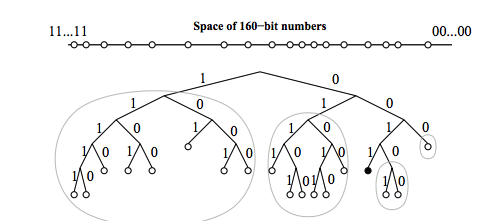
\includegraphics[width=0.6\textwidth]{kademlia}
  \caption[Kademlia Binary Tree]{Binary Tree zoals in gebruik bij het Kademlia protocol, \cite{maymounkov2002kademlia}.}
  \label{kademlia_binary_tree}
\end{wrapfigure}

Om het netwerk te betreden wordt er gebruik gemaakt van een bestaand protocol genaamd Kademlia, wat gebaseerd is op het gebruik van een \acrfull{DHT} architectuur. Elke node wordt behandeld als een tak in een Binary Tree waarbij de positie van een \gls{node} bepaald wordt door een unieke prefix van de identificatie code van een \gls{node}. In fig. \ref{kademlia_binary_tree} is de positie van een \gls{node} met de prefix 0011 te zien. Het protocol garandeert dat elke \gls{node} in verbinding staat met een andere \gls{node}. Met deze garantie kan elke \gls{node} een andere \gls{node} lokaliseren aan de hand van de identificatie code \citep[p.~2]{maymounkov2002kademlia}.

\subsubsection{Informatie propagatie}
Berichten worden verstuurd voor het uitwisselen van informatie tussen deelnemers. Hierbij zijn drie abstracte types gedefinieerd: \textit{inv}, \textit{req} en \textit{data}. Net zoals bij Bitcoin wordt de \textit{inv} message gebruikt om aan te geven dat er data beschikbaar is. Het \textit{req} bericht wordt vervolgens gebruikt om beschikbare data op te vragen. De data wordt vervolgens verstuurd via een \textit{data} message. Berichten die bijvoorbeeld een block versturen zijn nader gespecificeerde \textit{data} berichten. Op deze drie types zijn alle berichten in het netwerk gebaseerd, bijvoorbeeld is het \textit{MsgBlock} bericht, die block informatie uitwisselt, gebaseerd op een \textit{data} bericht \citep{cardano_wiki:csl_app_level}. Een bericht kan verstuurd worden naar drie verschillende mediums: het versturen van een bericht naar een \gls{node}, de buren, en het gehele netwerk. Naar welk medium het bericht wordt verstuurd is opgenomen in de header van een bericht.

\subsection{Gevaren}
\paragraph{Architectuur}
Net zoals bij Bitcoin zijn de transacties de kern van de implementatie, waarbij er wederom gebruik wordt gemaakt van het \gls{UTXO} zoals beschreven bij de architectuur van Bitcoin. 
De architectuur van het Cardano netwerk bestaat uit drie soorten \glspl{node} die fundamenteel zijn voor de werking van het protocol: \textit{core}, \textit{relay} en \textit{edge} \glspl{node}.\textit{Core \glspl{node}} zijn de kern van het netwerk. Het zijn de enige \glspl{node} die geselecteerd kunnen worden om \gls{slot_leader} te worden, waardoor het de enige \glspl{node} zijn die een block kunnen creëren.
\textit{Relay \glspl{node}} worden gezien als de proxy tussen core \glspl{node} en het internet. Ze hebben geen stake in het netwerk, waardoor ze makkelijk te verplaatsten of veranderd kunnen worden.
\textit{Edge \glspl{node}} zijn de simpele \glspl{node} die iedereen kan uitvoeren. Deze \glspl{node} kunnen transacties aanmaken binnen het netwerk en aanbieden aan \textit{core} \glspl{node} via de \textit{relay} \glspl{node} \citep[Topology]{cardano_wiki}.

\paragraph{Discovery protocol}
\begin{wrapfigure}{r}{0.6\textwidth}
  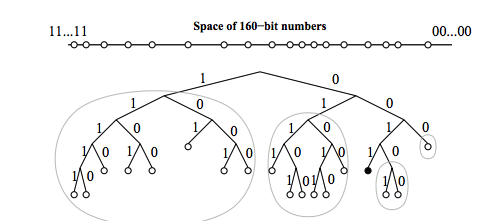
\includegraphics[width=0.6\textwidth]{kademlia}
  \caption[Kademlia Binary Tree]{Binary Tree zoals in gebruik bij het Kademlia protocol, \cite{maymounkov2002kademlia}.}
  \label{kademlia_binary_tree}
\end{wrapfigure}

Om het netwerk te betreden wordt er gebruik gemaakt van een bestaand protocol genaamd Kademlia, wat gebaseerd is op het gebruik van een \acrfull{DHT} architectuur. Elke node wordt behandeld als een tak in een Binary Tree waarbij de positie van een \gls{node} bepaald wordt door een unieke prefix van de identificatie code van een \gls{node}. In fig. \ref{kademlia_binary_tree} is de positie van een \gls{node} met de prefix 0011 te zien. Het protocol garandeert dat elke \gls{node} in verbinding staat met een andere \gls{node}. Met deze garantie kan elke \gls{node} een andere \gls{node} lokaliseren aan de hand van de identificatie code \citep[p.~2]{maymounkov2002kademlia}.

\subsubsection{Informatie propagatie}
Berichten worden verstuurd voor het uitwisselen van informatie tussen deelnemers. Hierbij zijn drie abstracte types gedefinieerd: \textit{inv}, \textit{req} en \textit{data}. Net zoals bij Bitcoin wordt de \textit{inv} message gebruikt om aan te geven dat er data beschikbaar is. Het \textit{req} bericht wordt vervolgens gebruikt om beschikbare data op te vragen. De data wordt vervolgens verstuurd via een \textit{data} message. Berichten die bijvoorbeeld een block versturen zijn nader gespecificeerde \textit{data} berichten. Op deze drie types zijn alle berichten in het netwerk gebaseerd, bijvoorbeeld is het \textit{MsgBlock} bericht, die block informatie uitwisselt, gebaseerd op een \textit{data} bericht \citep{cardano_wiki:csl_app_level}. Een bericht kan verstuurd worden naar drie verschillende mediums: het versturen van een bericht naar een \gls{node}, de buren, en het gehele netwerk. Naar welk medium het bericht wordt verstuurd is opgenomen in de header van een bericht.

\newpage
\subsection{Identiteit}
\paragraph{Architectuur}
Net zoals bij Bitcoin zijn de transacties de kern van de implementatie, waarbij er wederom gebruik wordt gemaakt van het \gls{UTXO} zoals beschreven bij de architectuur van Bitcoin. 
De architectuur van het Cardano netwerk bestaat uit drie soorten \glspl{node} die fundamenteel zijn voor de werking van het protocol: \textit{core}, \textit{relay} en \textit{edge} \glspl{node}.\textit{Core \glspl{node}} zijn de kern van het netwerk. Het zijn de enige \glspl{node} die geselecteerd kunnen worden om \gls{slot_leader} te worden, waardoor het de enige \glspl{node} zijn die een block kunnen creëren.
\textit{Relay \glspl{node}} worden gezien als de proxy tussen core \glspl{node} en het internet. Ze hebben geen stake in het netwerk, waardoor ze makkelijk te verplaatsten of veranderd kunnen worden.
\textit{Edge \glspl{node}} zijn de simpele \glspl{node} die iedereen kan uitvoeren. Deze \glspl{node} kunnen transacties aanmaken binnen het netwerk en aanbieden aan \textit{core} \glspl{node} via de \textit{relay} \glspl{node} \citep[Topology]{cardano_wiki}.

\paragraph{Discovery protocol}
\begin{wrapfigure}{r}{0.6\textwidth}
  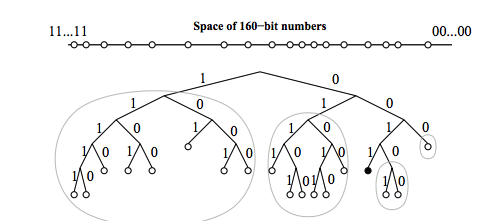
\includegraphics[width=0.6\textwidth]{kademlia}
  \caption[Kademlia Binary Tree]{Binary Tree zoals in gebruik bij het Kademlia protocol, \cite{maymounkov2002kademlia}.}
  \label{kademlia_binary_tree}
\end{wrapfigure}

Om het netwerk te betreden wordt er gebruik gemaakt van een bestaand protocol genaamd Kademlia, wat gebaseerd is op het gebruik van een \acrfull{DHT} architectuur. Elke node wordt behandeld als een tak in een Binary Tree waarbij de positie van een \gls{node} bepaald wordt door een unieke prefix van de identificatie code van een \gls{node}. In fig. \ref{kademlia_binary_tree} is de positie van een \gls{node} met de prefix 0011 te zien. Het protocol garandeert dat elke \gls{node} in verbinding staat met een andere \gls{node}. Met deze garantie kan elke \gls{node} een andere \gls{node} lokaliseren aan de hand van de identificatie code \citep[p.~2]{maymounkov2002kademlia}.

\subsubsection{Informatie propagatie}
Berichten worden verstuurd voor het uitwisselen van informatie tussen deelnemers. Hierbij zijn drie abstracte types gedefinieerd: \textit{inv}, \textit{req} en \textit{data}. Net zoals bij Bitcoin wordt de \textit{inv} message gebruikt om aan te geven dat er data beschikbaar is. Het \textit{req} bericht wordt vervolgens gebruikt om beschikbare data op te vragen. De data wordt vervolgens verstuurd via een \textit{data} message. Berichten die bijvoorbeeld een block versturen zijn nader gespecificeerde \textit{data} berichten. Op deze drie types zijn alle berichten in het netwerk gebaseerd, bijvoorbeeld is het \textit{MsgBlock} bericht, die block informatie uitwisselt, gebaseerd op een \textit{data} bericht \citep{cardano_wiki:csl_app_level}. Een bericht kan verstuurd worden naar drie verschillende mediums: het versturen van een bericht naar een \gls{node}, de buren, en het gehele netwerk. Naar welk medium het bericht wordt verstuurd is opgenomen in de header van een bericht.


\newpage

\section{EOS}
\subsection{Functionaliteit}
https://steemit.com/eos/@trogdor/eos-vs-ethereum-for-dummies

De blockchain implementatie EOS werkt toe naar een operating systeem speciaal voor blockchain toepassingen. In eerste instantie zal er een Blockchain gerealiseerd worden die dient als proof-of-concept van het ontwerp. In dit proof-of-concept is er een eerste versie gerealiseerd die het mogelijk maakt voor developers om een eigen applicatie op het EOS netwerk te creëren. Hierbij is de focus gelegd het faciliteren van functionaliteiten die betrekking hebben op account permissies, authenticatie en de communicatie tussen het internet en het netwerk. Er wordt gespeculeerd dat EOS een sterke concurrent van Ethereum zal worden als het gaat om Blockchain als een developer platform.

\paragraph{Architectuur}

EOS maakt gebruik van aanpak waarbij extensies op de basis componenten (e.g. het netwerk, de 'chain', etc.) gerealiseerd worden als plugins. Dit maakt het zodat het protocol makkelijk te wijzigen is in de toekomst. 
\paragraph{Discovery protocol}

\subsubsection{Informatie propagatie}
\subsection{Gevaren}
https://steemit.com/eos/@trogdor/eos-vs-ethereum-for-dummies

De blockchain implementatie EOS werkt toe naar een operating systeem speciaal voor blockchain toepassingen. In eerste instantie zal er een Blockchain gerealiseerd worden die dient als proof-of-concept van het ontwerp. In dit proof-of-concept is er een eerste versie gerealiseerd die het mogelijk maakt voor developers om een eigen applicatie op het EOS netwerk te creëren. Hierbij is de focus gelegd het faciliteren van functionaliteiten die betrekking hebben op account permissies, authenticatie en de communicatie tussen het internet en het netwerk. Er wordt gespeculeerd dat EOS een sterke concurrent van Ethereum zal worden als het gaat om Blockchain als een developer platform.

\paragraph{Architectuur}

EOS maakt gebruik van aanpak waarbij extensies op de basis componenten (e.g. het netwerk, de 'chain', etc.) gerealiseerd worden als plugins. Dit maakt het zodat het protocol makkelijk te wijzigen is in de toekomst. 
\paragraph{Discovery protocol}

\subsubsection{Informatie propagatie}
\subsection{Identiteit}
https://steemit.com/eos/@trogdor/eos-vs-ethereum-for-dummies

De blockchain implementatie EOS werkt toe naar een operating systeem speciaal voor blockchain toepassingen. In eerste instantie zal er een Blockchain gerealiseerd worden die dient als proof-of-concept van het ontwerp. In dit proof-of-concept is er een eerste versie gerealiseerd die het mogelijk maakt voor developers om een eigen applicatie op het EOS netwerk te creëren. Hierbij is de focus gelegd het faciliteren van functionaliteiten die betrekking hebben op account permissies, authenticatie en de communicatie tussen het internet en het netwerk. Er wordt gespeculeerd dat EOS een sterke concurrent van Ethereum zal worden als het gaat om Blockchain als een developer platform.

\paragraph{Architectuur}

EOS maakt gebruik van aanpak waarbij extensies op de basis componenten (e.g. het netwerk, de 'chain', etc.) gerealiseerd worden als plugins. Dit maakt het zodat het protocol makkelijk te wijzigen is in de toekomst. 
\paragraph{Discovery protocol}

\subsubsection{Informatie propagatie}

\section{Monero}
\subsection{Functionaliteit}
\paragraph{Architectuur}

Monero maakt gebruik van \acrfull{I2P} protocol. Het \acrshort{I2P} protocol stelt het netwerk in staat om deelnemers te beschermen tegen een zekere mate van verkeer; waarbij de identiteit van de verstuurder en ontvanger verborgen wordt, terwijl er gebruik gemaakt wordt van encryptiestandaarden om de inhoud van berichten te verbergen en te garanderen dat het bericht aankomt \citep{zantout2011i2p}. Het protocol ondersteund zowel TCP/IP als UDP/IP communicatie, waarbij de Transport laag in het network van Monero gelimiteerd is aan de mogelijkheden die \acrshort{I2P} ondersteund \citep{moneropedia:kovri}.
De transport laag faciliteert de connectie tussen de verschillende deelnemers in het netwerk. Om vervolgens te kunnen communiceren wordt er gebruik gemaakt van een \gls{tunnel}. Elke deelnemer in het netwerk heeft minimaal twee \Glspl{tunnel}, een voor uitgaand- en inkomend verkeer. Wanneer er communicatie plaatsvind tussen twee deelnemers zullen er vier \glspl{tunnel} aangemaakt worden; twee voor uitgaand verkeerd en twee voor inkomend verkeer \citep{moneropedia:tunnel}. Ook Monero maakt gebruik van het \gls{UTXO}, waarbij er bij iedere transactie twee keys aanwezig zijn; een spend key en een view key. Beide keys zijn onderdeel van een account, waarbij de spend key gebruikt wordt om geld uit te geven, en de view key gebruikt wordt om permissie te geven om de transacties in te zien van een deelnemer. De keys spelen een belangrijke rol in de privacy van de deelnemer omtrent transacties \citep{moneropedia:account}. 

\paragraph{Discovery protocol}

Het discovery protocol in gebruik bij Monero is soortgelijk aan de manier waarop Bitcoin het discovery proces uitvoert. Om het netwerk te bootstrappen wordt er gebruik gemaakt van \glspl{node} die vastgelegd zijn in de broncode, waarna er een lijst van \glspl{peer} wordt teruggegeven aan de deelnemer en de centrale node vergeten wordt. Het is ook mogelijk om zelf deelnemers vast te leggen waarna geprobeerd wordt om connectie te maken.

\paragraph{Informatie propagatie}

Alles binnen het \acrshort{I2P} netwerk wordt gecommuniceerd via berichten. In het onderdeel architectuur is er kort gesproken over \Gls{tunnel} en de functionaliteiten die ermee gerealiseerd wordt. Er zijn twee soorten berichten die verzonden worden: \Gls{tunnel} berichten en \acrfull{I2NP} berichten\footnote{Zie \href{https://geti2p.net/en/docs/protocol/i2np}{"I2NP Specifiation - I2P | Overview"} voor de verschillende types.}. Het proces, zoals beschreven in \cite{moneropedia:message}:

\begin{itemize}
  \setlength\itemsep{-0.7em}
  \item De \Gls{tunnel} verzameld \acrshort{I2NP} berichten en verwerkt ze naar \Gls{tunnel} berichten. Hierbij kan het voorkomen dat \acrshort{I2NP} berichten gefragmenteerd worden omdat ze van variabele grootte zijn, terwijl \Gls{tunnel} berichten een vaste grootte hebben.
  \item De \Gls{tunnel} encrypt de verwerkte data en stuurt het door in de vorm van \Gls{tunnel} berichten.
  \item De deelnemer, en andere deelnemers die deel uitmaken van de \Gls{tunnel}, pakken een laag van de encryptie uit en verifiëren dat het bericht geen duplicaat is en sturen het vervolgens door naar een volgende deelnemer.
  \item Met de tijd zullen de \Gls{tunnel} berichten het eindpunt bereiken waarna ze terug worden gezet naar de originele \acrshort{I2NP} berichten.
\end{itemize}
\subsection{Gevaren}
\paragraph{Architectuur}

Monero maakt gebruik van \acrfull{I2P} protocol. Het \acrshort{I2P} protocol stelt het netwerk in staat om deelnemers te beschermen tegen een zekere mate van verkeer; waarbij de identiteit van de verstuurder en ontvanger verborgen wordt, terwijl er gebruik gemaakt wordt van encryptiestandaarden om de inhoud van berichten te verbergen en te garanderen dat het bericht aankomt \citep{zantout2011i2p}. Het protocol ondersteund zowel TCP/IP als UDP/IP communicatie, waarbij de Transport laag in het network van Monero gelimiteerd is aan de mogelijkheden die \acrshort{I2P} ondersteund \citep{moneropedia:kovri}.
De transport laag faciliteert de connectie tussen de verschillende deelnemers in het netwerk. Om vervolgens te kunnen communiceren wordt er gebruik gemaakt van een \gls{tunnel}. Elke deelnemer in het netwerk heeft minimaal twee \Glspl{tunnel}, een voor uitgaand- en inkomend verkeer. Wanneer er communicatie plaatsvind tussen twee deelnemers zullen er vier \glspl{tunnel} aangemaakt worden; twee voor uitgaand verkeerd en twee voor inkomend verkeer \citep{moneropedia:tunnel}. Ook Monero maakt gebruik van het \gls{UTXO}, waarbij er bij iedere transactie twee keys aanwezig zijn; een spend key en een view key. Beide keys zijn onderdeel van een account, waarbij de spend key gebruikt wordt om geld uit te geven, en de view key gebruikt wordt om permissie te geven om de transacties in te zien van een deelnemer. De keys spelen een belangrijke rol in de privacy van de deelnemer omtrent transacties \citep{moneropedia:account}. 

\paragraph{Discovery protocol}

Het discovery protocol in gebruik bij Monero is soortgelijk aan de manier waarop Bitcoin het discovery proces uitvoert. Om het netwerk te bootstrappen wordt er gebruik gemaakt van \glspl{node} die vastgelegd zijn in de broncode, waarna er een lijst van \glspl{peer} wordt teruggegeven aan de deelnemer en de centrale node vergeten wordt. Het is ook mogelijk om zelf deelnemers vast te leggen waarna geprobeerd wordt om connectie te maken.

\paragraph{Informatie propagatie}

Alles binnen het \acrshort{I2P} netwerk wordt gecommuniceerd via berichten. In het onderdeel architectuur is er kort gesproken over \Gls{tunnel} en de functionaliteiten die ermee gerealiseerd wordt. Er zijn twee soorten berichten die verzonden worden: \Gls{tunnel} berichten en \acrfull{I2NP} berichten\footnote{Zie \href{https://geti2p.net/en/docs/protocol/i2np}{"I2NP Specifiation - I2P | Overview"} voor de verschillende types.}. Het proces, zoals beschreven in \cite{moneropedia:message}:

\begin{itemize}
  \setlength\itemsep{-0.7em}
  \item De \Gls{tunnel} verzameld \acrshort{I2NP} berichten en verwerkt ze naar \Gls{tunnel} berichten. Hierbij kan het voorkomen dat \acrshort{I2NP} berichten gefragmenteerd worden omdat ze van variabele grootte zijn, terwijl \Gls{tunnel} berichten een vaste grootte hebben.
  \item De \Gls{tunnel} encrypt de verwerkte data en stuurt het door in de vorm van \Gls{tunnel} berichten.
  \item De deelnemer, en andere deelnemers die deel uitmaken van de \Gls{tunnel}, pakken een laag van de encryptie uit en verifiëren dat het bericht geen duplicaat is en sturen het vervolgens door naar een volgende deelnemer.
  \item Met de tijd zullen de \Gls{tunnel} berichten het eindpunt bereiken waarna ze terug worden gezet naar de originele \acrshort{I2NP} berichten.
\end{itemize}
\subsection{Identiteit}
\paragraph{Architectuur}

Monero maakt gebruik van \acrfull{I2P} protocol. Het \acrshort{I2P} protocol stelt het netwerk in staat om deelnemers te beschermen tegen een zekere mate van verkeer; waarbij de identiteit van de verstuurder en ontvanger verborgen wordt, terwijl er gebruik gemaakt wordt van encryptiestandaarden om de inhoud van berichten te verbergen en te garanderen dat het bericht aankomt \citep{zantout2011i2p}. Het protocol ondersteund zowel TCP/IP als UDP/IP communicatie, waarbij de Transport laag in het network van Monero gelimiteerd is aan de mogelijkheden die \acrshort{I2P} ondersteund \citep{moneropedia:kovri}.
De transport laag faciliteert de connectie tussen de verschillende deelnemers in het netwerk. Om vervolgens te kunnen communiceren wordt er gebruik gemaakt van een \gls{tunnel}. Elke deelnemer in het netwerk heeft minimaal twee \Glspl{tunnel}, een voor uitgaand- en inkomend verkeer. Wanneer er communicatie plaatsvind tussen twee deelnemers zullen er vier \glspl{tunnel} aangemaakt worden; twee voor uitgaand verkeerd en twee voor inkomend verkeer \citep{moneropedia:tunnel}. Ook Monero maakt gebruik van het \gls{UTXO}, waarbij er bij iedere transactie twee keys aanwezig zijn; een spend key en een view key. Beide keys zijn onderdeel van een account, waarbij de spend key gebruikt wordt om geld uit te geven, en de view key gebruikt wordt om permissie te geven om de transacties in te zien van een deelnemer. De keys spelen een belangrijke rol in de privacy van de deelnemer omtrent transacties \citep{moneropedia:account}. 

\paragraph{Discovery protocol}

Het discovery protocol in gebruik bij Monero is soortgelijk aan de manier waarop Bitcoin het discovery proces uitvoert. Om het netwerk te bootstrappen wordt er gebruik gemaakt van \glspl{node} die vastgelegd zijn in de broncode, waarna er een lijst van \glspl{peer} wordt teruggegeven aan de deelnemer en de centrale node vergeten wordt. Het is ook mogelijk om zelf deelnemers vast te leggen waarna geprobeerd wordt om connectie te maken.

\paragraph{Informatie propagatie}

Alles binnen het \acrshort{I2P} netwerk wordt gecommuniceerd via berichten. In het onderdeel architectuur is er kort gesproken over \Gls{tunnel} en de functionaliteiten die ermee gerealiseerd wordt. Er zijn twee soorten berichten die verzonden worden: \Gls{tunnel} berichten en \acrfull{I2NP} berichten\footnote{Zie \href{https://geti2p.net/en/docs/protocol/i2np}{"I2NP Specifiation - I2P | Overview"} voor de verschillende types.}. Het proces, zoals beschreven in \cite{moneropedia:message}:

\begin{itemize}
  \setlength\itemsep{-0.7em}
  \item De \Gls{tunnel} verzameld \acrshort{I2NP} berichten en verwerkt ze naar \Gls{tunnel} berichten. Hierbij kan het voorkomen dat \acrshort{I2NP} berichten gefragmenteerd worden omdat ze van variabele grootte zijn, terwijl \Gls{tunnel} berichten een vaste grootte hebben.
  \item De \Gls{tunnel} encrypt de verwerkte data en stuurt het door in de vorm van \Gls{tunnel} berichten.
  \item De deelnemer, en andere deelnemers die deel uitmaken van de \Gls{tunnel}, pakken een laag van de encryptie uit en verifiëren dat het bericht geen duplicaat is en sturen het vervolgens door naar een volgende deelnemer.
  \item Met de tijd zullen de \Gls{tunnel} berichten het eindpunt bereiken waarna ze terug worden gezet naar de originele \acrshort{I2NP} berichten.
\end{itemize}